\documentclass{standalone}
\usepackage{tikz}
\usetikzlibrary{patterns, positioning}


\begin{document}
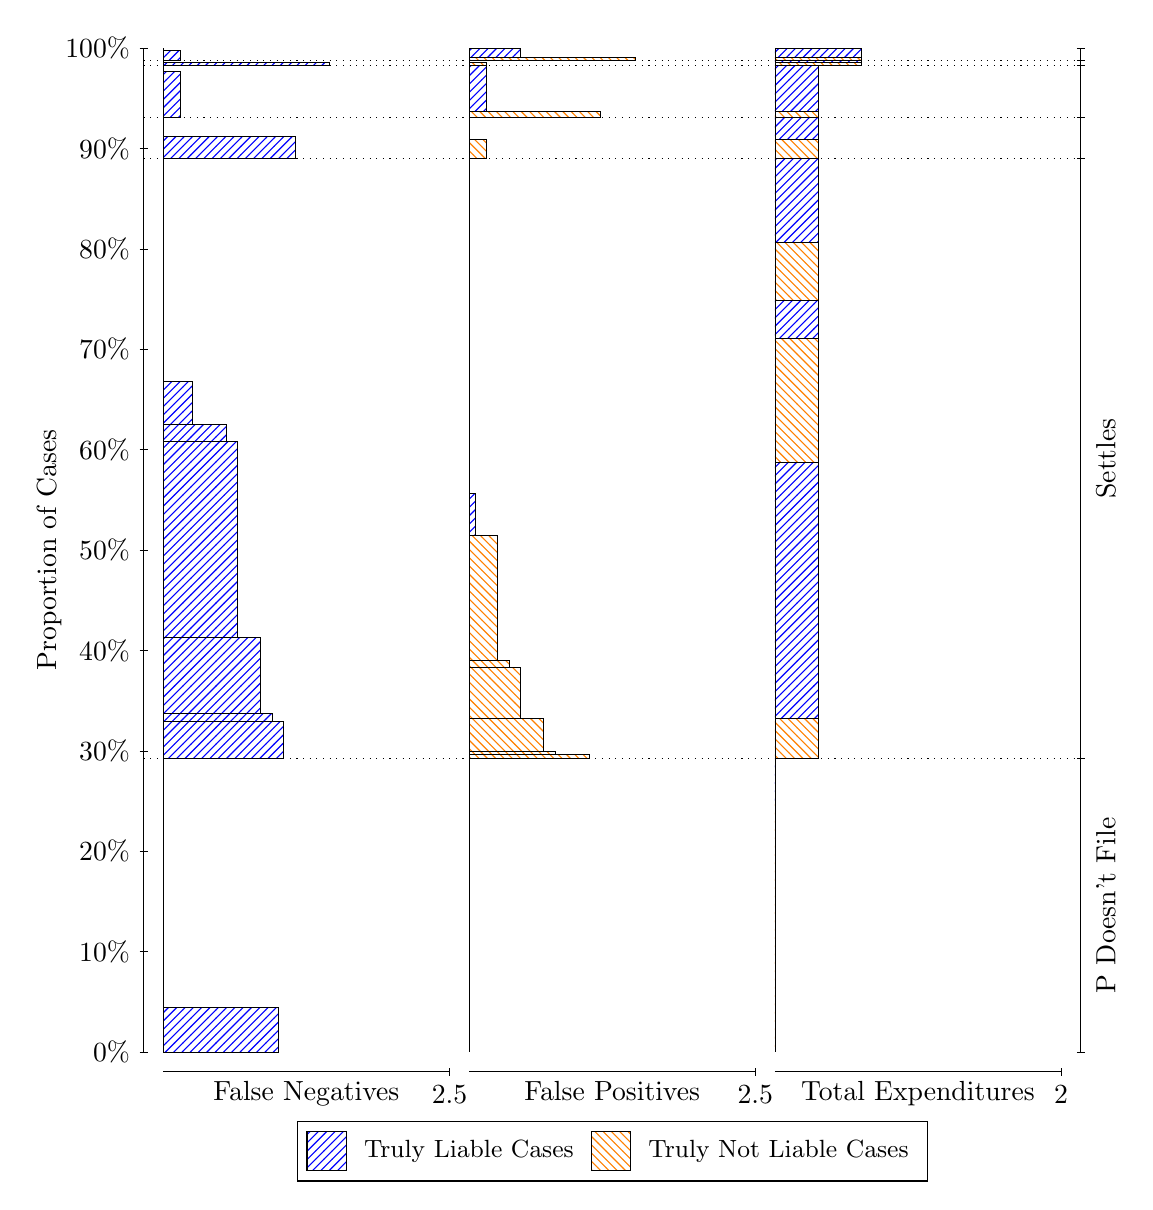
\begin{tikzpicture}
\draw[black, very thin] (1.5,1.75) -- (1.5,14.5);
\node[rotate=90, text=black, anchor=center] at (0.3, 8.125) {Proportion of Cases};
\draw[black, very thin] (1.45,1.75) -- (1.55,1.75);
\node[text=black, anchor=east] at (1.45, 1.75) {0\%};
\draw[black, very thin] (1.45,3.025) -- (1.55,3.025);
\node[text=black, anchor=east] at (1.45, 3.025) {10\%};
\draw[black, very thin] (1.45,4.3) -- (1.55,4.3);
\node[text=black, anchor=east] at (1.45, 4.3) {20\%};
\draw[black, very thin] (1.45,5.575) -- (1.55,5.575);
\node[text=black, anchor=east] at (1.45, 5.575) {30\%};
\draw[black, very thin] (1.45,6.85) -- (1.55,6.85);
\node[text=black, anchor=east] at (1.45, 6.85) {40\%};
\draw[black, very thin] (1.45,8.125) -- (1.55,8.125);
\node[text=black, anchor=east] at (1.45, 8.125) {50\%};
\draw[black, very thin] (1.45,9.4) -- (1.55,9.4);
\node[text=black, anchor=east] at (1.45, 9.4) {60\%};
\draw[black, very thin] (1.45,10.675) -- (1.55,10.675);
\node[text=black, anchor=east] at (1.45, 10.675) {70\%};
\draw[black, very thin] (1.45,11.95) -- (1.55,11.95);
\node[text=black, anchor=east] at (1.45, 11.95) {80\%};
\draw[black, very thin] (1.45,13.225) -- (1.55,13.225);
\node[text=black, anchor=east] at (1.45, 13.225) {90\%};
\draw[black, very thin] (1.45,14.5) -- (1.55,14.5);
\node[text=black, anchor=east] at (1.45, 14.5) {100\%};

\draw[black, very thin] (13.4,1.75) -- (13.4,14.5);
\draw[black, very thin] (13.35,1.75) -- (13.45,1.75);
\node[anchor=west] at (13.35, 1.75) {};
\draw[black, very thin] (13.35,5.4764) -- (13.45,5.4764);
\node[anchor=west] at (13.35, 5.4764) {};
\draw[black, very thin] (13.35,13.096) -- (13.45,13.096);
\node[anchor=west] at (13.35, 13.096) {};
\draw[black, very thin] (13.35,13.615) -- (13.45,13.615);
\node[anchor=west] at (13.35, 13.615) {};
\draw[black, very thin] (13.35,14.282) -- (13.45,14.282);
\node[anchor=west] at (13.35, 14.282) {};
\draw[black, very thin] (13.35,14.347) -- (13.45,14.347);
\node[anchor=west] at (13.35, 14.347) {};
\draw[black, very thin] (13.35,14.5) -- (13.45,14.5);
\node[anchor=west] at (13.35, 14.5) {};

\draw[black, very thin, pattern color=blue, pattern=north east lines] (1.75,1.75) rectangle (3.2033,2.312);
\draw[black, very thin, pattern color=orange, pattern=north west lines] (1.75,2.312) rectangle (1.75,5.4764);
\draw[black, very thin, pattern color=blue, pattern=north east lines] (1.75,5.4764) rectangle (3.276,5.9527);
\draw[black, very thin, pattern color=blue, pattern=north east lines] (1.75,5.9527) rectangle (3.1307,6.0527);
\draw[black, very thin, pattern color=blue, pattern=north east lines] (1.75,6.0527) rectangle (2.9853,7.0176);
\draw[black, very thin, pattern color=blue, pattern=north east lines] (1.75,7.0176) rectangle (2.6947,9.5008);
\draw[black, very thin, pattern color=blue, pattern=north east lines] (1.75,9.5008) rectangle (2.5493,9.7242);
\draw[black, very thin, pattern color=blue, pattern=north east lines] (1.75,9.7242) rectangle (2.1133,10.266);
\draw[black, very thin, pattern color=orange, pattern=north west lines] (1.75,10.266) rectangle (1.75,13.096);
\draw[black, very thin, pattern color=blue, pattern=north east lines] (1.75,13.096) rectangle (3.4213,13.375);
\draw[black, very thin, pattern color=orange, pattern=north west lines] (1.75,13.375) rectangle (1.75,13.615);
\draw[black, very thin, pattern color=blue, pattern=north east lines] (1.75,13.615) rectangle (1.968,14.206);
\draw[black, very thin, pattern color=orange, pattern=north west lines] (1.75,14.206) rectangle (1.75,14.282);
\draw[black, very thin, pattern color=blue, pattern=north east lines] (1.75,14.282) rectangle (3.8573,14.313);
\draw[black, very thin, pattern color=orange, pattern=north west lines] (1.75,14.313) rectangle (1.75,14.347);
\draw[black, very thin, pattern color=blue, pattern=north east lines] (1.75,14.347) rectangle (1.968,14.468);
\draw[black, very thin, pattern color=orange, pattern=north west lines] (1.75,14.468) rectangle (1.75,14.5);
\draw[black, very thin, pattern color=orange, pattern=north west lines] (5.6333,1.75) rectangle (5.6333,4.9144);
\draw[black, very thin, pattern color=blue, pattern=north east lines] (5.6333,4.9144) rectangle (5.6333,5.4764);
\draw[black, very thin, pattern color=orange, pattern=north west lines] (5.6333,5.4764) rectangle (7.1593,5.5311);
\draw[black, very thin, pattern color=orange, pattern=north west lines] (5.6333,5.5311) rectangle (6.7233,5.5656);
\draw[black, very thin, pattern color=orange, pattern=north west lines] (5.6333,5.5656) rectangle (6.578,5.9877);
\draw[black, very thin, pattern color=orange, pattern=north west lines] (5.6333,5.9877) rectangle (6.2873,6.6349);
\draw[black, very thin, pattern color=orange, pattern=north west lines] (5.6333,6.6349) rectangle (6.142,6.7274);
\draw[black, very thin, pattern color=orange, pattern=north west lines] (5.6333,6.7274) rectangle (5.9967,8.3058);
\draw[black, very thin, pattern color=blue, pattern=north east lines] (5.6333,8.3058) rectangle (5.706,8.8481);
\draw[black, very thin, pattern color=blue, pattern=north east lines] (5.6333,8.8481) rectangle (5.6333,13.096);
\draw[black, very thin, pattern color=orange, pattern=north west lines] (5.6333,13.096) rectangle (5.8513,13.335);
\draw[black, very thin, pattern color=blue, pattern=north east lines] (5.6333,13.335) rectangle (5.6333,13.615);
\draw[black, very thin, pattern color=orange, pattern=north west lines] (5.6333,13.615) rectangle (7.3047,13.691);
\draw[black, very thin, pattern color=blue, pattern=north east lines] (5.6333,13.691) rectangle (5.8513,14.282);
\draw[black, very thin, pattern color=orange, pattern=north west lines] (5.6333,14.282) rectangle (5.8513,14.315);
\draw[black, very thin, pattern color=blue, pattern=north east lines] (5.6333,14.315) rectangle (5.6333,14.347);
\draw[black, very thin, pattern color=orange, pattern=north west lines] (5.6333,14.347) rectangle (7.7407,14.379);
\draw[black, very thin, pattern color=blue, pattern=north east lines] (5.6333,14.379) rectangle (6.2873,14.5);
\draw[black, very thin, pattern color=orange, pattern=north west lines] (9.5167,1.75) rectangle (9.5167,4.9144);
\draw[black, very thin, pattern color=blue, pattern=north east lines] (9.5167,4.9144) rectangle (9.5167,5.4764);
\draw[black, very thin, pattern color=orange, pattern=north west lines] (9.5167,5.4764) rectangle (10.062,5.9877);
\draw[black, very thin, pattern color=blue, pattern=north east lines] (9.5167,5.9877) rectangle (10.062,9.2364);
\draw[black, very thin, pattern color=orange, pattern=north west lines] (9.5167,9.2364) rectangle (10.062,10.815);
\draw[black, very thin, pattern color=blue, pattern=north east lines] (9.5167,10.815) rectangle (10.062,11.291);
\draw[black, very thin, pattern color=orange, pattern=north west lines] (9.5167,11.291) rectangle (10.062,12.031);
\draw[black, very thin, pattern color=blue, pattern=north east lines] (9.5167,12.031) rectangle (10.062,13.096);
\draw[black, very thin, pattern color=orange, pattern=north west lines] (9.5167,13.096) rectangle (10.062,13.335);
\draw[black, very thin, pattern color=blue, pattern=north east lines] (9.5167,13.335) rectangle (10.062,13.615);
\draw[black, very thin, pattern color=orange, pattern=north west lines] (9.5167,13.615) rectangle (10.062,13.691);
\draw[black, very thin, pattern color=blue, pattern=north east lines] (9.5167,13.691) rectangle (10.062,14.282);
\draw[black, very thin, pattern color=orange, pattern=north west lines] (9.5167,14.282) rectangle (10.607,14.315);
\draw[black, very thin, pattern color=blue, pattern=north east lines] (9.5167,14.315) rectangle (10.607,14.347);
\draw[black, very thin, pattern color=orange, pattern=north west lines] (9.5167,14.347) rectangle (10.607,14.379);
\draw[black, very thin, pattern color=blue, pattern=north east lines] (9.5167,14.379) rectangle (10.607,14.5);
\draw[black, dotted] (1.5,5.4764) -- (13.4,5.4764);
\draw[black, dotted] (1.5,13.096) -- (13.4,13.096);
\draw[black, dotted] (1.5,13.615) -- (13.4,13.615);
\draw[black, dotted] (1.5,14.282) -- (13.4,14.282);
\draw[black, dotted] (1.5,14.347) -- (13.4,14.347);
\draw[black, very thin] (1.75,1.5) -- (5.3833,1.5);
\node[text=black, anchor=north] at (3.5667, 1.5) {False Negatives};
\draw[black, very thin] (5.3833,1.45) -- (5.3833,1.55);
\node[text=black, anchor=north] at (5.3833, 1.45) {2.5};

\draw[black, very thin] (5.6333,1.5) -- (9.2667,1.5);
\node[text=black, anchor=north] at (7.45, 1.5) {False Positives};
\draw[black, very thin] (9.2667,1.45) -- (9.2667,1.55);
\node[text=black, anchor=north] at (9.2667, 1.45) {2.5};

\draw[black, very thin] (9.5167,1.5) -- (13.15,1.5);
\node[text=black, anchor=north] at (11.333, 1.5) {Total Expenditures};
\draw[black, very thin] (13.15,1.45) -- (13.15,1.55);
\node[text=black, anchor=north] at (13.15, 1.45) {2};

\node[text=black, centered, rotate=90] at (13.72, 3.6132) {P Doesn't File};
\node[text=black, centered, rotate=90] at (13.72, 9.2861) {Settles};





\draw (7.449999999999999,1.5) node[draw=none] (baseCoordinate) {};
\begin{scope}[align=center]
        \matrix[scale=0.5, draw=black, below=0.5cm of baseCoordinate, nodes={draw}, column sep=0.1cm]{
            \node[rectangle, draw, minimum width=0.5cm, minimum height=0.5cm, pattern color=blue, pattern=north east lines] {}; &
            \node[draw=none, font=\small, text=black] (B) {Truly Liable Cases}; &
            \node[rectangle, draw, minimum width=0.5cm, minimum height=0.5cm, pattern color=orange, pattern=north west lines] {}; &
            \node[draw=none, font=\small, text=black] (B) {Truly Not Liable Cases}; \\
            };
\end{scope}

\end{tikzpicture}
\end{document}